\section{Gecombineerde effecten en verdere voorspellingen}

Nu we afzonderlijke tijdsdilatatiefactoren hebben afgeleid voor beweging door æther en gravitationele ætherstroom, beschouwen we beide effecten nu tegelijkertijd.

\subsection*{Gecombineerde beweging en gravitationeel veld}

Laat een wervelklok bewegen met snelheid $\vec{u}$ in een gebied waar de æther stroomt met snelheid $\vec{v}_g$. De effectieve relatieve snelheid ten opzichte van de lokale ætherstroom is:
\[
    \vec{v}_{\text{rel}} = \vec{u} - \vec{v}_g.
\]
De waargenomen tijdsdilatatie is dan:
\[
    \frac{d\tau}{dt} = \sqrt{1 - \frac{|\vec{v}_{\text{rel}}|^2}{c^2}}. \tag{5}
\]
Deze formulering integreert zowel speciale als algemene relativistische effecten op soepele wijze in één enkele uitdrukking.

\subsection*{Voorbeeld: Circulaire baantijdsdilatatie}

Beschouw een klok die rond een massa $M$ draait met straal $r$. De tangentiële snelheid van de baan is:
\[
    v_{\text{orb}} = \sqrt{\frac{GM}{r}}, \quad v_g(r) = \sqrt{\frac{2GM}{r}}.
\]
Aangezien de baansnelheid loodrecht staat op de radiale ætherinstroom, is de relatieve snelheid:
\[
    v_{\text{rel}} = \sqrt{v_{\text{orb}}^2 + v_g^2} = \sqrt{\frac{3GM}{r}}.
\]

\begin{figure}[htbp]
    \centering
    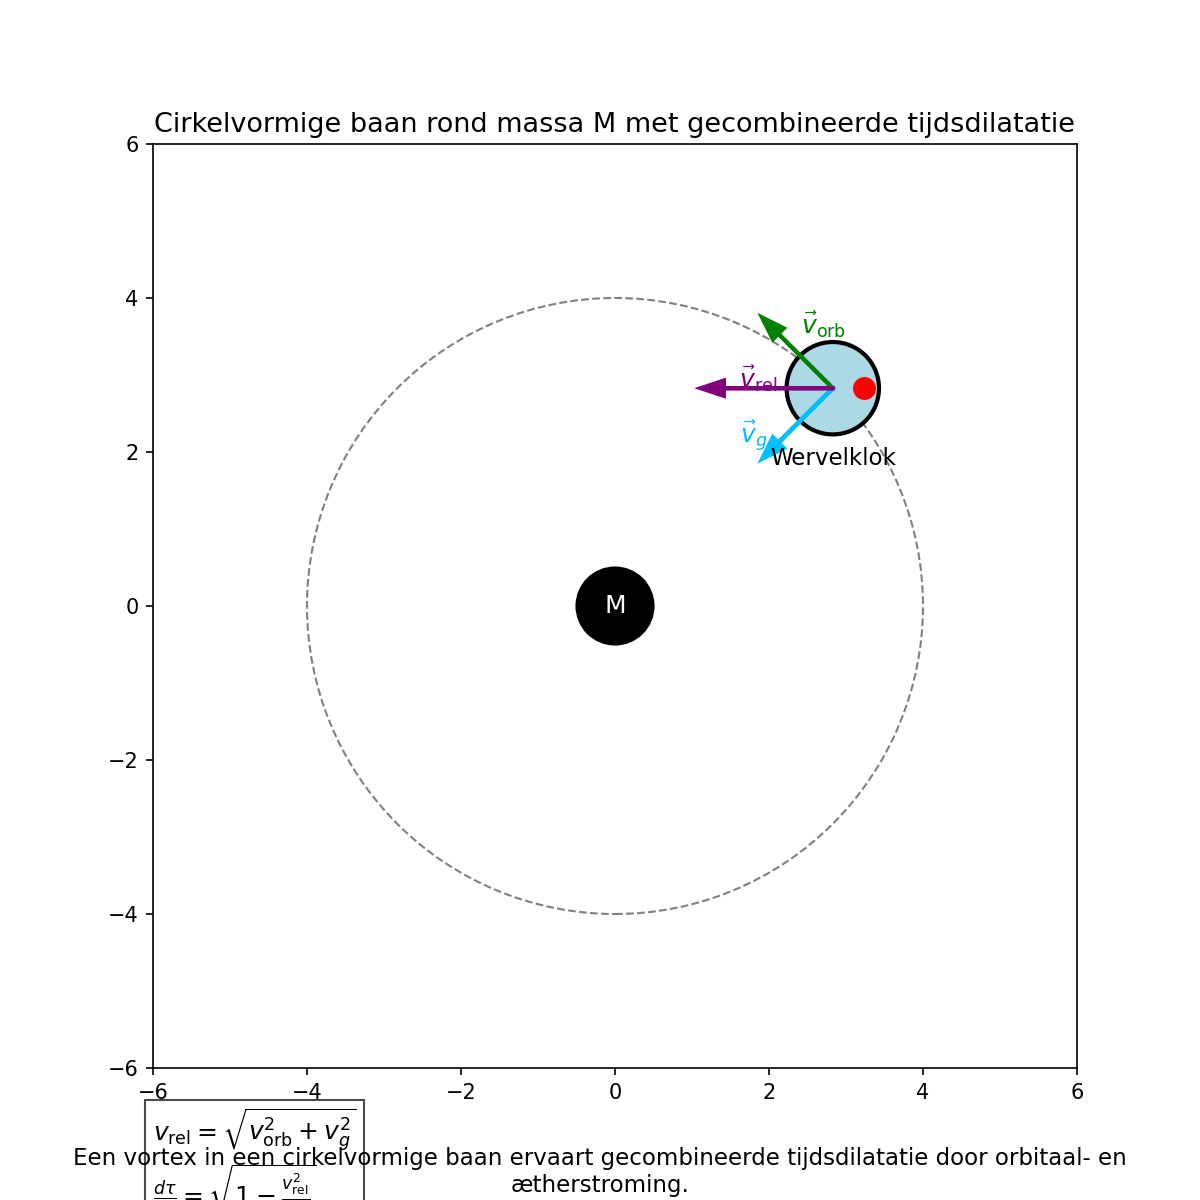
\includegraphics[width=0.85\textwidth]{5-BaanRondMassa}
    \caption{.}
    \label{fig:BaanRondMassa}
\end{figure}


De tijdsdilatatie wordt dus:
\[
    \frac{d\tau}{dt} = \sqrt{1 - \frac{3GM}{rc^2}}. \tag{6}
\]
Dit komt overeen met het exacte resultaat van Schwarzschild-geometrie voor cirkelvormige banen.

\subsection*{Implicaties nabij een horizon}

Als $r \to r_s = 2GM/c^2$ nadert de instroomsnelheid $v_g(r)$ $c$ en vertraagt de klok van elke statische waarnemer tot nul. De ætherstroom onderdrukt de lokale wervelrotatie volledig, wat een natuurlijk mechanisme biedt voor het \("\)bevriezen van de tijd\("\) aan de gebeurtenishorizon.


\begin{figure}[htbp]
    \centering
    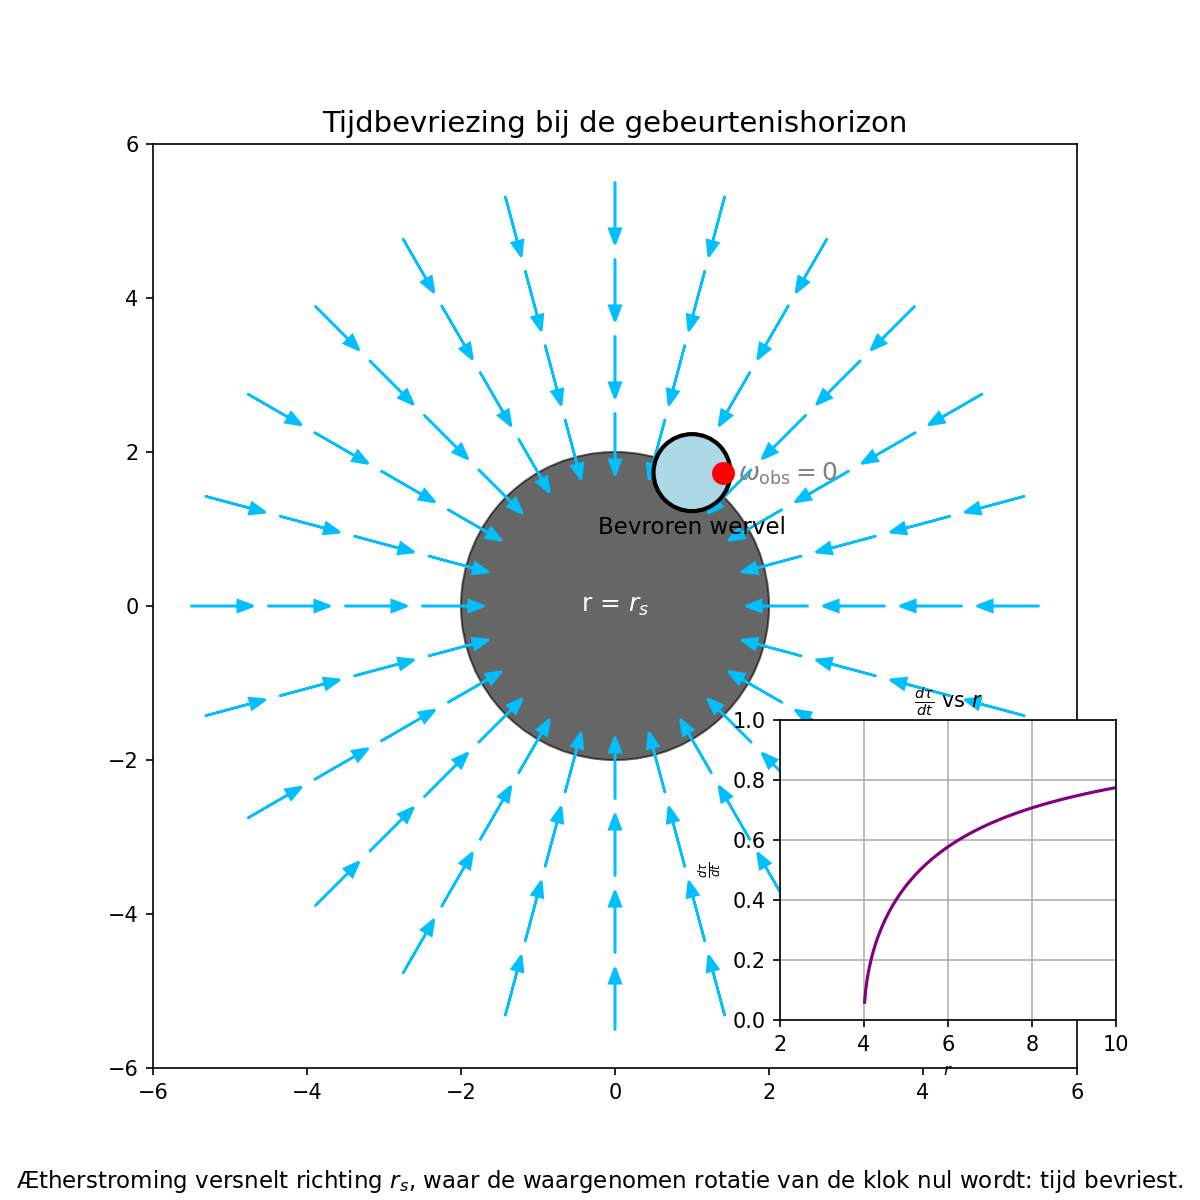
\includegraphics[width=0.85\textwidth]{6-HorizonTijdsbevriezing}
    \caption{.}
    \label{fig:HorizonTijdsbevriezing}
\end{figure}

\subsection*{Uniforme interpretatie}

Dit æthermodel maakt het mogelijk om alle relativistische tijdsdilatatie-effecten te zien als gevolgen van één principe:
\[
    \text{Kloksnelheidsreductie} \;\propto\; \text{relatieve beweging door æther}.
\]
Of deze relatieve beweging nu voortkomt uit traagheidssnelheid of uit ætherische instroom vanwege nabijgelegen massa, het waarneembare gevolg is hetzelfde. Daarom concluderen we:
\[
    \boxed{\frac{d\tau}{dt} = \sqrt{1 - \frac{|\vec{u} - \vec{v}_g|^2}{c^2}}}
\]
als de algemene tijdsdilatatieformule voor het Vortex Æther Model.


\begin{figure}[htbp]
    \centering
    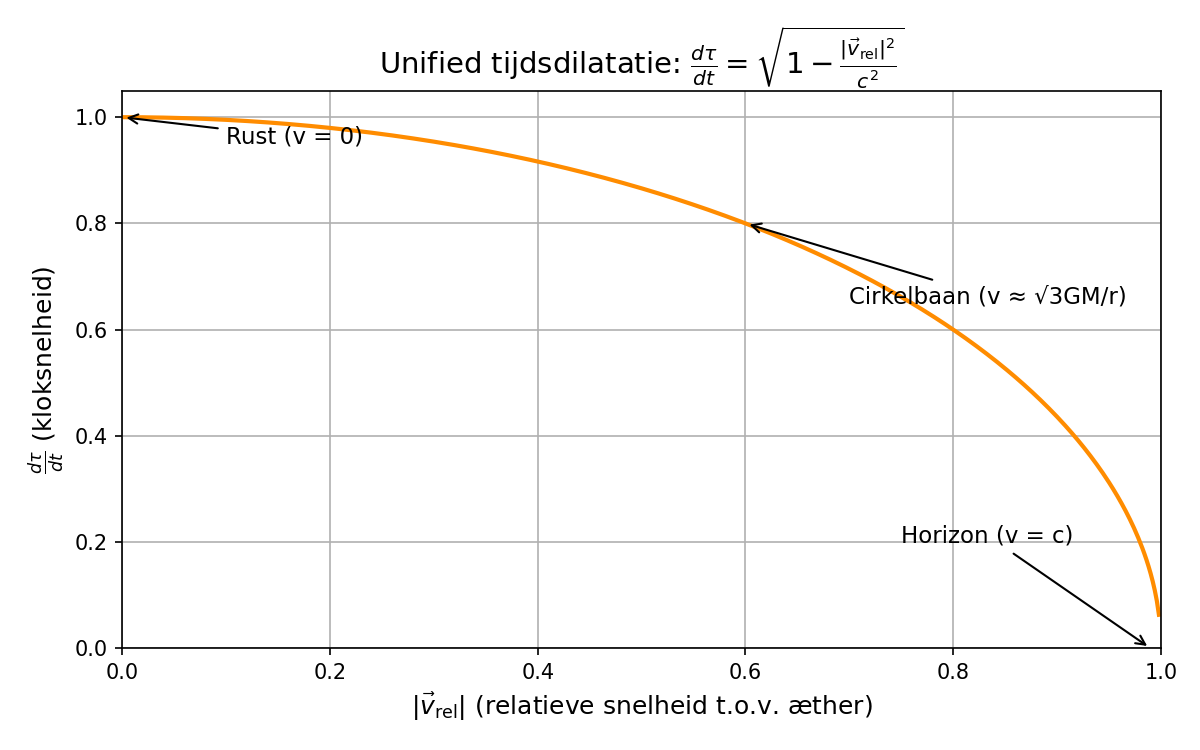
\includegraphics[width=0.85\textwidth]{7-TijdsvertragingRelatieveBeweging}
    \caption{.}
    \label{fig:TijdsvertragingRelatieveBeweging}
\end{figure}

Voor mogelijke experimentele afwijkingen van deze tijdsdilatatieformules t.o.v. de algemene relativiteitstheorie, zie Appendix~\ref{appendix:AfwijkendeVoorspellingen}.